\documentclass[12pt]{article}
\usepackage{graphicx}
\usepackage{xcolor}
% \usepackage[margin=1.7cm]{geometry}
\usepackage{colortbl}
\usepackage{tikz}
\usepackage{amsmath}
\usepackage{caption}
\usepackage{subcaption}
\usepackage{textcomp}
\usepackage{float}
\usepackage{alltt}
\renewcommand{\ttdefault}{txtt}
\newcommand{\todo}[2]{{\color{red}\textbf{Todo voor #1:} #2}}
\begin{document}
\begin{titlepage}
\begin{center}
    
\includegraphics[width=\textwidth]{./logo.png}
    \\ [2.5cm]
    \textsc{\Large Inleiding Modelleren en Simuleren}
    \\ [0.5cm]
    \textsc{\large Final Assignment}
    \\ [1cm]
    \hrule
    \vspace{0.3cm}
    \textsc{N-body simulator}
    \\ [0.3cm]
    \hrule
    \vfill
    \textsc{David van Erkelens, 10264019 \\[0.7cm] Department of Computer Science \\ University of Amsterdam \\[0.4cm] \today \\[0.5cm] Alle code ook beschikbaar op}
    \\
    \verb|www.github.com/David1209/N-Body-Simulator|
\end{center}
\end{titlepage}
\tableofcontents
\clearpage
\section{Inleiding}
Al sinds de tijd van de oude Grieken houdt men zich bezig met het bestuderen van de sterren. Met behulp van een N-body simulator kan de beweging van onder andere sterren, maar ook moleculen en andere lichamen welke invloed op elkaar uitoefenen gesimuleerd worden. In 1687 formuleerde Sir Isaac Newton de principes welke ten gronde liggen aan de aantrekkingskracht tussen twee lichamen. Hoewel Newton niet in staat was dit op de lossen voor meer dan twee lichamen, valt dit wel te benaderen met behulp van numerieke simulaties.
\section{Formules}
Om te berekenen welke invloed de verschillende lichamen op elkaar hebben, worden Newtons wetten van beweging en aantrekkingskracht gebruikt. Voor dit systeem wordt er vanuit gegaan dat voor ieder lichaam de beginpositie $(p_x, p_y)$ en beginsnelheid $(v_x, v_y)$ bekend zijn. Om vervolgens de dynamica van het systeem te kunnen bekijken, moet de kracht welke vanuit andere lichamen op het lichaam uitgeoefend wordt, worden doorgerekend. Om dit te kunnen doen, worden de volgende wetten van Newton toegepast:
\begin{itemize}
\item \textbf{Paarsgewijze kracht:} volgens Newtons wet van universele aantrekkingskracht wordt de aantrekkingskracht tussen twee lichamen beschreven door het product van hun massa's, gedeeld door het kwadraat van de afstand tussen hen: 
\begin{equation}
F = \frac{Gm_1m_2}{r^2}
\end{equation}
waarin G de gravitationele constante is, welke de waarde $G = 6.67 \times 10^{-11} N \frac{m^2}{kg^2}$ heeft. 
\item \textbf{Netto kracht:} volgens het principe van superpositie is de netto kracht op een lichaam gelijk aan de som van de paarsgewijze krachten van alle lichamen op het lichaam.
\item \textbf{Versnelling:} volgens Newtons tweede wet van beweging wordt de versnelling van een lichaam gegeven door $a = \frac{F}{m}$.
\end{itemize}
\section{Implementatie}
Om de N-body simulator te implementeren, is er gebruik gemaakt van Java. Aangezien Java een object-ge\"orienteerde programmeertaal is, is het heel logisch om voor ieder lichaam een apart object aan te maken. 
\subsection{Body-object}
In \verb|Body.java| wordt het object voor alle lichamen aangemaakt. Ieder lichaam heeft meerdere eigenschappen:
\begin{itemize}
\item Een $(x, y)$ positie.
\item Een $(v_x, v_y)$ versnelling.
\item Een massa.
\item Een kleur om het lichaam in de simulatie te tekenen.
\item De straal van het lichaam in de simulatie.
\item Een \verb|ArrayList| met de geschiedenis om een lijn achter het lichaam te kunnen tekenen.
\end{itemize}
Naast "getters" en "setters" voor bovenstaande eigenschappen, bevat de klasse nog de volgende functies:
\begin{itemize}
\item \verb|update()|: deze voert een tijdstap door en verplaatst een lichaam naar een nieuwe locatie
\item \verb|getDistance(Body b)|: berekent de afstand tussen het huidige lichaam en meegegeven lichaam \verb|b|
\item Constructor \verb|Body| waaraan de tekenstraal, locatie, versnelling en massa meegegeven worden.
\end{itemize}
\subsection{BodyPanel klasse}
Om de lichamen in de simulatie te kunnen tekenen, wordt de \verb|BodyPanel| klasse gebruikt. Deze klasse is een uitbreiding van \verb|JPanel|. Deze klasse bevat de volgende variabelen:
\begin{itemize}
\item \verb|bodies|, een \verb|ArrayList| met daarin alle lichamen welke getekend moeten worden (van de klasse \verb|Body|).
\item \verb|worldsize|, de grootte van het universum waarin alle lichamen zich bevinden.
\item \verb|windowsize|, de grootte van het scherm waarin de simulatie uitgevoerd wordt.
\end{itemize}
Daarnaast bevat de klasse de volgende functies:
\begin{itemize}
\item \verb|paintComponent|, een functie welke iedere keer als \verb|.repaint()| aangeroepen wordt de nieuwe locatie van de lichamen tekent.
\item \verb|world2screen|, een functie welke het universum schaalt en transleert om in het scherm te passen.
\item Constructor \verb|BodyPanel| waaraan de \verb|ArrayList| met lichamen, universumgrootte en schermgrootte meegegeven worden.
\end{itemize}
\subsection{nBodySimulator}
In \verb|nBodySimulator.java| wordt de daadwerkelijke simulatie uitgevoerd. Omdat de \verb|Body| klasse werkt met Cartesiaanse co\"ordinaten, is het handig om de berekeningen van kracht en versnelling om te schrijven naar losse berekeningen langs de assen. Dit geeft:
\begin{equation}
	F_x = F\frac{{\delta}x}{r}
\end{equation}
\begin{equation}
	F_y = F\frac{{\delta}y}{r}
\end{equation}
voor de kracht, en
\begin{equation}
	a_x = \frac{F_x}{m}
	\label{ax}
\end{equation}
\begin{equation}
	a_y = \frac{F_y}{m}
	\label{ay}
\end{equation}
voor de versnelling. Omdat $G$ een onafhankelijke constante is, wordt deze versimpeld naar de vorm:
\begin{equation}
	G = 6.67 \times 10^{-11}
\end{equation}
Nu deze gegevens bekend zijn, worden voor ieder lichaam $F_x$ en $F_y$ berekend. Hierbij moet opgemerkt worden dat het teken in ${\delta}x$ en ${\delta}y$ van belang is, deze afstanden worden berekend door de co\"ordinaten van het huidige lichaam in mindering te brengen bij de co\"ordinaten van het lichaam waarmee de kracht berekend wordt:
\begin{equation}
	\begin{pmatrix} {\delta}x \\
	{\delta}y
	\end{pmatrix}
	= 
	\begin{pmatrix} x \\
	y
	\end{pmatrix}_{ander lichaam}
	- 
	\begin{pmatrix} x \\
	y
	\end{pmatrix}_{huidig lichaam}
\end{equation}
Nu $F_x$ en $F_y$ berekend zijn, kan de versnelling met behulp van formules \ref{ax} en \ref{ay} berekend worden. Er vanuit gaande dat de versnelling constant is in de grootte van de tijdstap, wordt de nieuwe versnelling van het lichaam gegeven door:
\begin{equation}
	\begin{pmatrix}v_x + {\delta}t \times a_x \\
	v_y + {\delta}t \times a_y
	\end{pmatrix}
\end{equation}
Waarin ${\delta}t$ is vastgesteld op $5 \times 10^5$. Aan de hand van deze versnelling kan de nieuwe locatie berekend worden. In \verb|nBodySimulator.java| is dit als volgt ge\"implementeerd (pseudocode):
\begin{alltt}
\textbf{for} ieder lichaam:
    \textbf{for} iedere ander lichaam:
        berekend afstand;
        bereken force in x en y richting;
    tel alle x en y force bij elkaar op;
    bereken de nieuwe versnelling;
    stel de nieuwe versnelling in;

\textbf{for} ieder lichaam:
    verplaats het lichaam;
\end{alltt}
Het verplaatsen van het lichaam wordt in een nieuwe loop geplaatst, omdat eerst de oude positie van het lichaam voor ieder ander lichaam doorgerekend moet worden voordat het lichaam verplaatst kan worden.
\clearpage
\section{Experimenten}
Met de N-body simulator zijn twee experimenten uitgevoerd, een met twee symmetrische planeten welke om elkaar heen draaien en een met de helft van ons zonnestelsel.
\subsection{Symmetrische planeten}
Voor dit experiment zijn de volgende lichamen gebruikt: \\[0.2cm]
\begin{tabular}{| l | c | c | c | c |}
	\hline
	& Startpositie & Startsnelheid & Massa & Kleur \\
	\hline
	Lichaam 1 & $(0, 4.5e10)$ & $(1.0e7, 0)$ & $1.5e30$ & Blauw \\
	\hline
	Lichaam 2 & $(0, -4.5e10)$ & $(-1.0e7, 0)$ & $1.5e30$ & Rood \\
	\hline
\end{tabular} \\[0.2cm]
Deze twee lichamen hebben dezelfde eigenschappen en blijven eeuwig om elkaar heen draaien, doordat deze telkens weer tot elkaar aangetrokken worden. Door de gelijke eigenschappen vertoont deze simulatie een symmetrisch uiterlijk. Dit experiment valt uit te voeren met het commando \verb|java | \\
\verb|nBodySimulator two|.
\begin{figure}[h!]
	\centering
	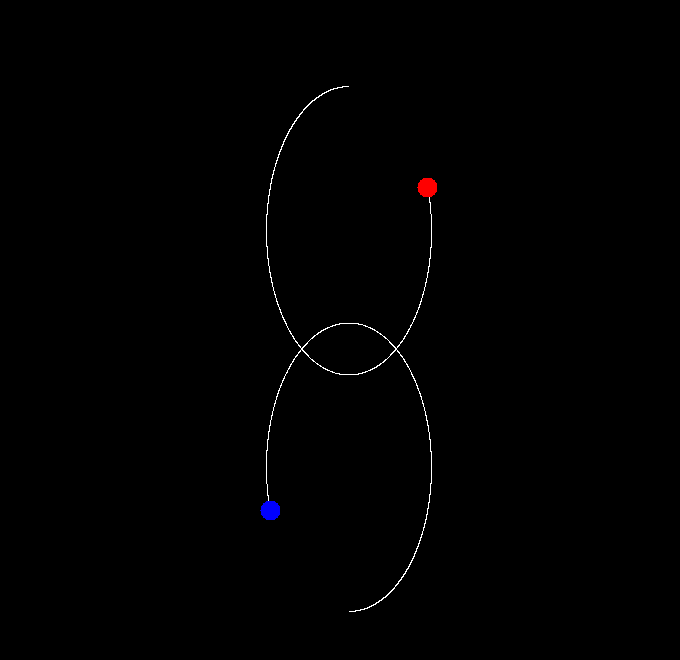
\includegraphics[width=0.6\textwidth]{2plan.png}
	\caption{Twee planeten welke om elkaar heen draaien}
	\label{twee}
\end{figure}
\subsection{Zonnestelsel}
Voor dit experiment zijn de volgende lichamen gebruikt:\footnote{Data afkomstig van www.cs.princeton.edu/courses/archive/fall13/cos126/assignments/nbody.html} \\[0.2cm]
\begin{tabular}{| l | c | c | c | c |}
	\hline
	& Startpositie & Startsnelheid & Massa & Kleur \\
	\hline
	Zon & $(0, 0)$ & $(0, 0)$ & $1.989e30$ & Geel \\
	\hline
	Mercurius & $(5.79e10, 0)$ & $(0, 4.79e7)$ & $3.302e23$ & Oranje \\
	\hline
	Venus & $(1.082e11, 0)$ & $(0, 3.5e7)$ & $4.869e24$ & Roze \\
	\hline
	Aarde & $(1.496e11, 0)$ & $(0, 2.98e7)$ & $5.9740e24$ & Blauw \\
	\hline
	Mars & $(2.279e11, 0)$ & $(0, 2.41e7)$ & $6,419e23$ & Rood \\
	\hline
\end{tabular} \\[0.2cm]
In dit experiment komt de aantrekkingskracht van de zon mooi naar voren. Doordat de zon een enorme massa heeft in vergelijking met de andere planeten, blijft zelfs de meest ver weg liggende planeet (Mars) om de zon heen draaien. Ondanks dat de planeten onderling ook invloed op elkaar hebben, valt dit te verwaarlozen in vergelijking met de invloed van de zwaartekracht van de zon. Dit experiment valt uit te voeren door de simulator zonder argumenten te starten.
\begin{figure}[h!]
	\centering
	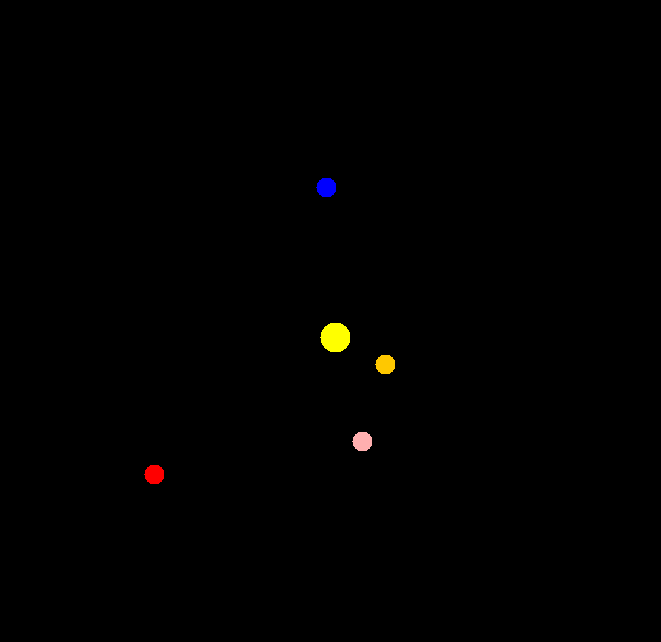
\includegraphics[width=0.6\textwidth]{solar.png}
	\caption{Het halve zonnestelsel}
	\label{zonne}
\end{figure}
\section{Beperkingen}
De grootste beperking van de N-body simulator is de preciezie. Doordat N-body simulaties voor $N > 2$ alleen te benaderen zijn en niet exact op te lossen, zal het resultaat van de simulator altijd een benadering zijn en nooit het exacte antwoord. Een verdere beperking in de implementatie van de N-body simulator valt te zien in het verschil tussen afbeelding \ref{twee} en \ref{zonne}. In afbeelding \ref{twee} worden er nog afgelegde banen achter de lichamen getekend, maar in afbeelding \ref{zonne} niet. Dit valt te verklaren doordat de \verb|ArrayList| waarin de geschiedenis van de lichamen bewaard worden na een tijd behoorlijk groot wordt, en hierdoor de simulatie zwaar vertraagd. Dit valt in de toekomst op te lossen door alleen het laatste stuk van de staart te tekenen of de staart met mindere precieze te tekenen.
\section{Conclusie}
Er valt te concluderen dat de N-body simulator goed werkt. Planeten laten duidelijk hun samenhang zien en de simulator loopt soepel. Ruimte voor verbetering is er nog door meer experimenten te doen en het probleem met het tekenen van de staart op te lossen. N-body simulaties blijken een redelijk natuurgetrouwe manier te zijn om samenhang tussen lichamen weer te geven, maar door het gebrek aan een volledige wiskunde oplossing zal het nooit een exacte beschrijving van de natuur zijn.
\end {document}